\chapter{Theoretical Model}
\label{ch:theoretical-model}

In this chapter we cover the structure of the codebook transfer model, as provided by Li \textit{et al.} \cite{10.5555/1661445.1661773}, and explore the variant proposed by Zang \textit{et al.}, called LKT-FM \cite{10.1007/978-3-319-71246-8_39}.


\section{Codebook Transfer (CBT)}

CBT is a cross-domain recommender system aiming to transfer the rating pattern from a source domain to a target domain, to improve data quantity and provide better recommendations in the target domain. According to Li \textit{et al.} \cite{10.5555/1661445.1661773} CBT \textquote{can transfer useful knowledge from the auxiliary rating matrix in some other domains to remedy the sparsity of the rating matrix in a target domain}.\\
Due to the nature of the model, we can distinguish three phases: codebook construction, codebook transfer and top-k recommendation.


\subsection{Input Data}

Input data provided to the CBT model consists in two user-rating matrices. We call $URM_S$ the user-rating matrix of the source domain and $URM_T$ the user-rating matrix of the target domain.\\
While no user or item overlap is not required, CBT has only requirement for input data: the sparsity of the source dataset should be low enough to allow a meaningful amount of knowledge to be transferred. In \cite{10.5555/1661445.1661773} Li \textit{et al.} did not provide a functional sparsity percentage. In their experiment, the source dataset had a sparsity lower than 50\%.


\subsection{Codebook Construction}

Codebook construction exploits the assumption that, in CF, users with similar tastes or items with similar attributes behave similarly. For this reason, it is possible to compute user and item clusters to obtain a much more compact user-rating matrix of the source domain, which represents the groups behavior. The obtained compact user-rating matrix is called \textit{codebook}.\\
Li \textit{et al.} provided the following definition for \textit{codebook}:
\begin{displayquote}
\enquote{Codebook is a $k \times l$ matrix which compresses the cluster-level user-item rating patterns of $k$ user clusters and $l$ item clusters in the original rating matrix.}
\end{displayquote}
Once the codebook has been computed, an approximation of the original user-rating matrix can be retrieved.\par
The codebook construction has to be performed by clustering users and items simultaneously. The authors adopted ONMTF \cite{10.1145/1150402.1150420} as the clustering algorithm. Thus, given a source user-rating matrix $X_S$ with shape $n \times m$ and a target codebook size $k \times l$, the optimization problem is the following:
\begin{equation}
\min_{U_S \in \mathbb{R}^{n \times k}_+, V_S \in \mathbb{R}^{m \times l}_+, S \in \mathbb{R}^{k \times l}_+} \norm{X_S - U_S S V_S^T}_F^2, \quad \text{s.t.} \quad U_S^T U_S = I, V_S^T V_S = I
\end{equation}
Where $U_S$ is the matrix of user clusters indicators and $V_S$ is the matrix of item clusters indicators.\\
$U_S$, $V_S$ and $S$ can be initialized randomly or with K-Means.\\
Since it is sufficient to obtain a cluster hard membership indicator for each user and item, $U_S$ and $V_S$ are binarized to have only the non-negative entry in each row set to 1 and the others set to 0.\\
Once $U_S$ and $V_S$ are computed, the codebook $B$ is computed as follows:
\begin{equation}
\label{eq:codebook-construction}
B = \frac{U_S^T X_S V_S}{U_S^T 11^T V_S}
\end{equation}
The complete algorithm for codebook construction is the following:
\vskip 0.7cm
\begin{algorithm}[H]
\SetKwInOut{Input}{Input}
\SetKwInOut{Output}{Output}
\Input{The source domain user-rating matrix $X_S \in \mathbb{R}^{n \times m}$;\\
The amount of user and item clusters $k$ and $l$.}
\Output{A codebook $B \in \mathbb{R}^{k \times l}$ learned from $X_S$.}
Initialize $U_S^{(0)}$, $V_S^{(0)}$, $S^{(0)}$ randomly or with K-Means\;
\For{$t \gets 1$ \KwTo $max\_iteration$}
{
  Update $U_S$, $V_S$ and $S$ using the following equations:\\
  $V_S^{(t)} \gets V_S^{(t - 1)} \odot \sqrt{\frac{X_S^T U_S^{(t - 1)} S^{(t - 1)}}{V_S^{(t - 1)} [V_S^{(t - 1)}]^T X_S^T U_S^{(t - 1)} S^{(t - 1)}}}$\;
  $U_S^{(t)} \gets U_S^{(t - 1)} \odot \sqrt{\frac{X_S V_S^{(t)} [S^{(t - 1)}]^T}{U_S^{(t - 1)} [U_S^{(t - 1)}]^T X_S V_S^{(t)} [S^{(t - 1)}]^T}}$\;
  $S^{(t)} \gets S^{(t - 1)} \odot \sqrt{\frac{[U_S^{(t)}]^T X_S V_S^{(t)}}{[U_S^{(t)}]^T U_S^{(t)} S^{(t - 1)} [V_S^{(t)}]^T V_S^{(t)}}}$\;
}
Allocate spaces for $U_S$ and $V_S$\;
\For{$i \gets 1$ \KwTo $n$}
{
  $\hat{j} = argmax_{j \in (1,...,k)}(U_{ij})$\;
  $[U_S]_{i\hat{j}} \gets 1$\;
  \For{$j \in (1,...,k)/\hat{j}$}
  {
    $[U_S]_{ij} \gets 0$\;
  }
}
\For{$i \gets 1$ \KwTo $m$}
{
  $\hat{j} = argmax_{j \in (1,...,l)}(V_{ij})$\;
  $[V_S]_{i\hat{j}} \gets 1$\;
  \For{$j \in (1,...,l)/\hat{j}$}
  {
    $[V_S]_{ij} \gets 0$\;
  }
}
Compute $B$ using \autoref{eq:codebook-construction}:\\
$B = \frac{U_S^T X_S V_S}{U_S^T 11^T V_S}$;
\caption{The algorithm for codebook construction}
\end{algorithm}
\vskip 0.7cm
According to Li \textit{et al.}, too many clusters can comprise redundant information, while too few cluster could be insufficient to encode the users and items information, missing important knowledge. An optimal codebook size should be expressive enough and suitable for computation.
\begin{figure}[hbt]
  \centering
  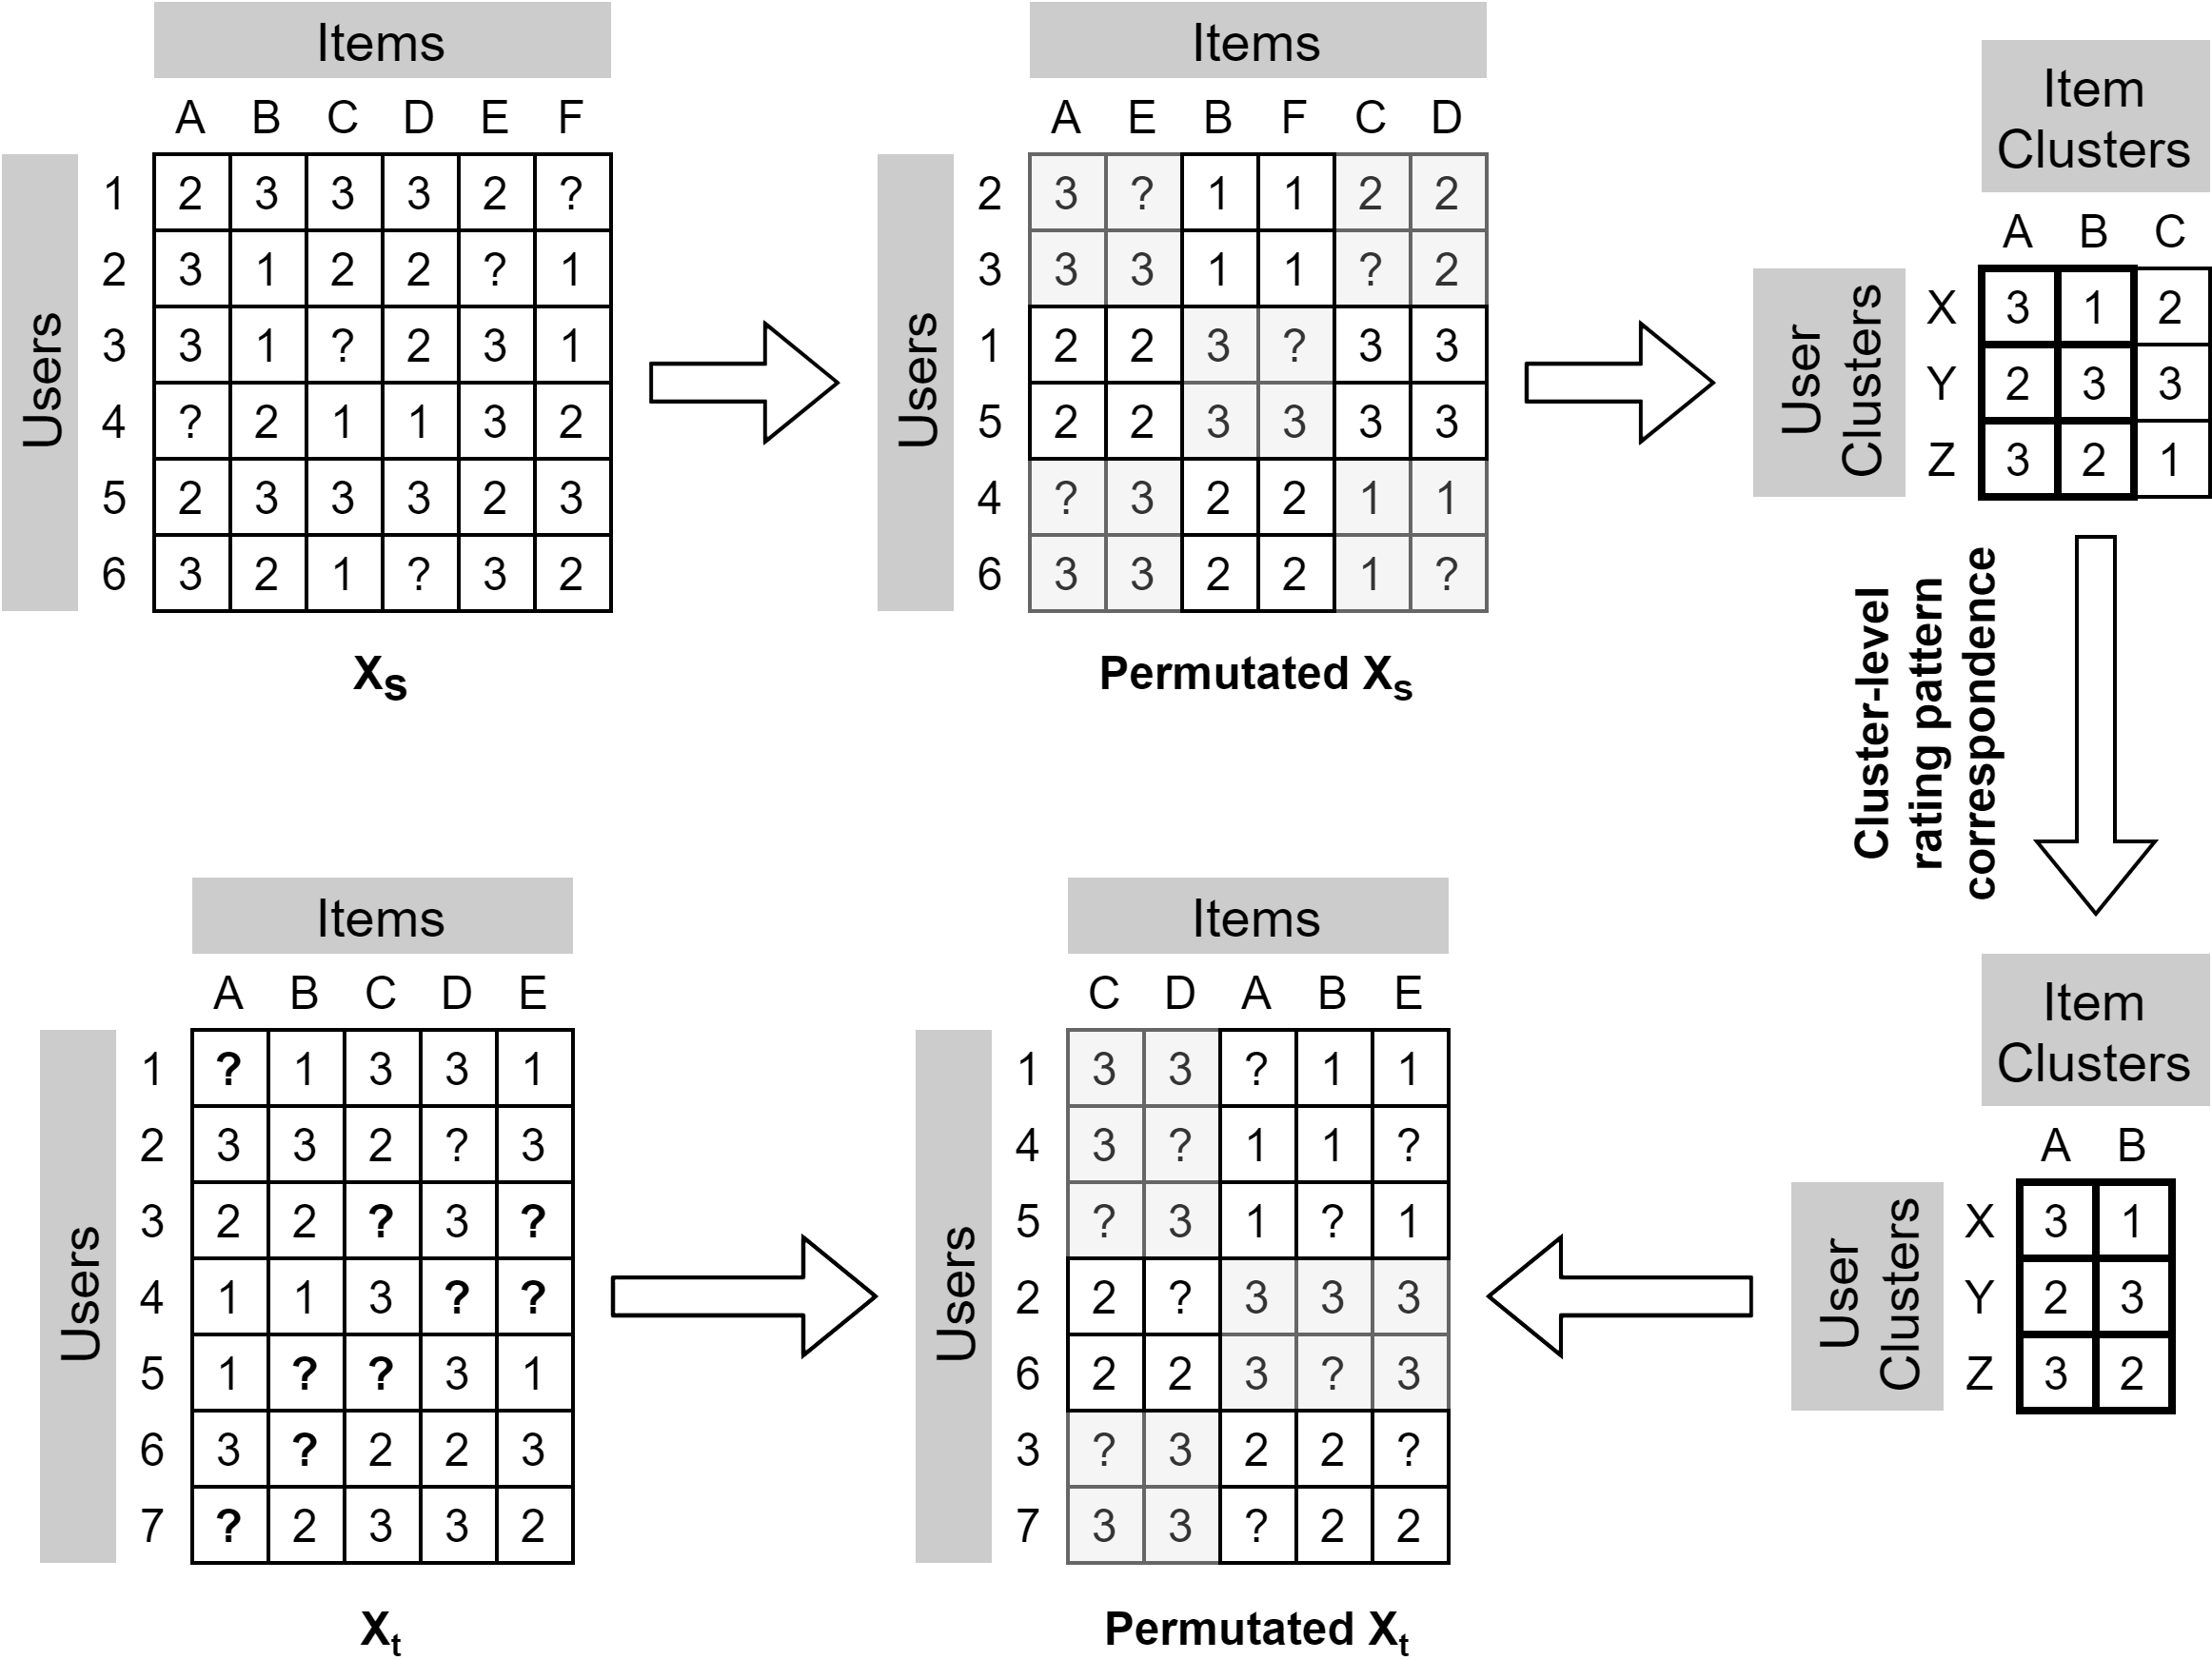
\includegraphics[width=0.8\textwidth]{pictures/codebook-construction}
  \caption
  [Example of codebook construction. Source: https://dl.acm.org/doi/10.5555/1661445.1661773]
  {\protect\raggedright Example of codebook construction. Source: https://dl.acm.org/doi/10.5555/1661445.1661773}
\end{figure}


\subsection{Codebook Transfer}
\label{sc:codebook-transfer}

\begin{figure}[hbt]
  \centering
  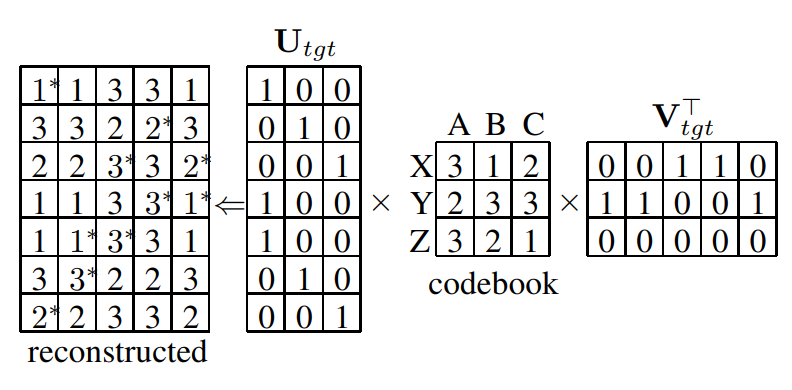
\includegraphics[width=0.8\textwidth]{pictures/codebook-transfer}
  \caption
  [Example of codebook transfer. Source: https://dl.acm.org/doi/10.5555/1661445.1661773]
  {\protect\raggedright Example of codebook transfer. Source: https://dl.acm.org/doi/10.5555/1661445.1661773}
\end{figure}
Having constructed the codebook $B$, the model applies it to the target domain. To do this, it assumes that there is correspondence of user and item clusters between the two domains. Transferring the rating pattern consists in the inverse operation to codebook construction. The codebook is expanded to reconstruct an approximation of the target user-rating matrix $X_T$.\\
The duplication of a row or column of the codebook implies that there is a set of users or items in the target domain that behaves like the cluster represented by the row or column.\\
Once an approximation of $X_T$ has been obtained, it is suitable to exclude the already observed ratings in order to predict only the missing entries.\\
The minimization problem for codebook transfer is defined as follows:
\begin{equation}
\min_{U_T \in \{0,1\}^{p \times k}, V_T \in \{0,1\}^{q \times l}} \norm{[X_T - U_T B V_T^T] \odot W}_F^2, \quad \text{s.t.} \quad U_T 1 = 1, V_T 1 = 1
\end{equation}
where $U_T$ and $V_T$ are the matrices of cluster membership, respectively for users and items, such that:
\begin{equation}
[U_T]_{ij} =
\begin{cases}
0, & \text{if user}\ [X_T]_{i}\ \text{belongs to cluster}\ j\\
1, & \text{otherwise}
\end{cases}
, \quad \text{s.t.} \quad i \in \{1,p\}, j \in \{1,k\}
\end{equation}
\begin{equation}
[V_T]_{ij} =
\begin{cases}
0, & \text{if item}\ [X_T]_{i}\ \text{belongs to cluster}\ j\\
1, & \text{otherwise}
\end{cases}
, \quad \text{s.t.} \quad i \in \{1,q\}, j \in \{1,l\}
\end{equation}
and $W$ is the masking matrix with shape $p \times q$ such that:
\begin{equation}
W_{ij} =
\begin{cases}
0, & \text{if}\ [X_T]_{ij}\ \text{is not rated}\\
1, & \text{otherwise}
\end{cases}
, \quad \text{s.t.} \quad i \in \{1,p\}, j \in \{1,q\}
\end{equation}
Once $U_T$ and $V_T$ have been obtained, it is possible to expand the codebook and fill the target user-rating matrix as follows:
\begin{equation}
\label{eq:codebook-transfer-fill}
\bar{X_T} = W \odot X_T + [1 - W] \odot [U_T B V_T^T]
\end{equation}
The complete algorithm for codebook transfer is the following:
\vskip 0.7cm
\begin{algorithm}[H]
\SetKwInOut{Input}{Input}
\SetKwInOut{Output}{Output}
\Input{The codebook $B \in \mathbb{R}^{k \times l}$ learned from $X_S$;\\
The target domain user-rating matrix $X_T \in \mathbb{R}^{p \times q}$;\\
The masking matrix $W \in \{0,1\}^{p \times q}$.}
\Output{The filled target domain user-rating matrix $\bar{X_T}$.}
Allocate spaces for $U_S$ and $V_S$\;
\For{$i \gets 1$ \KwTo $m$}
{
  $\hat{j} =\ \text{random from}\ \{1,...,l\}$\;
  $[V_T^{(0)}]_{i\hat{j}} \gets 1$\;
  \For{$j \in (1,...,l)/\hat{j}$}
  {
    $[V_T^{(0)}]_{ij} \gets 0$\;
  }
}
\For{$t \gets 1$ \KwTo $max\_iteration$}
{
  \For{$i \gets 1$ \KwTo $p$}
  {
    $\hat{j} = argmin_j \norm{[X_T]_{i*} - [B [V_T^{(t - 1)}]^T]_{j*}}_{W_{i*}}^2$\;
    $[U_T^{(t)}]_{i\hat{j}} \gets 1$\;
    \For{$j \in (1,...,k)/\hat{j}$}
    {
      $[U_T^{(t)}]_{ij} \gets 0$\;
    }
  }
  \For{$i \gets 1$ \KwTo $q$}
  {
    $\hat{j} = argmin_j \norm{[X_T]_{*i} - {[U_T^{(t - 1)} B]}_{*j}}_{W_{*i}}^2$\;
    $[V_T^{(t)}]_{i\hat{j}} \gets 1$\;
    \For{$j \in (1,...,l)/\hat{j}$}
    {
      $[V_T^{(t)}]_{ij} \gets 0$\;
    }
  }
}
Compute $X_T$ using \autoref{eq:codebook-transfer-fill}:
$\bar{X_T} = W \odot X_T + [1 - W] \odot [U_T B V_T^T]$\;
\caption{The algorithm for codebook transfer}
\label{al:codebook-transfer}
\end{algorithm}
\vskip 0.7cm
The following passages prove that the codebook transfer algorithm monotically reduces the loss function. In particular it needs to be proved that the following inequalities always hold:
\begin{equation}
\label{eq:codebook-transfer-monotone-1}
\begin{split}
& \norm{[X_T - U_T^{(t - 1)} B [V_T^{(t - 1)}]^T] \odot W}_F^2 \\
\geq & \norm{[X_T - U_T^{(t)} B [V_T^{(t - 1)}]^T] \odot W}_F^2
\end{split}
\end{equation}
\begin{equation}
\label{eq:codebook-transfer-monotone-2}
\begin{split}
& \norm{[X_T - U_T^{(t)} B [V_T^{(t - 1)}]^T] \odot W}_F^2 \\
\geq & \norm{[X_T - U_T^{(t)} B [V_T^{(t)}]^T] \odot W}_F^2
\end{split}
\end{equation}
First, the authors prove \autoref{eq:codebook-transfer-monotone-1}, where $U_T$ is updated and $V_T$ is fixed. It is possible to state that:
\begin{equation}
\label{eq:codebook-transfer-monotone-3}
\begin{split}
& \norm{[X_T - U_T^{(t - 1)} B [V_T^{(t - 1)}]^T] \odot W}_F^2 \\
= & \sum_{i = 1}^{n} \sum_{j = 1}^{k} [U_T^{(t - 1)}]_{ij} \norm{[X_T]_{i*} - [B [V_T^{(t - 1)}]^T]_{j*}}_{W_{i*}}^2 \\
= & \sum_{i = 1}^{n} \norm{[X_T]_{i*} - [B [V_T^{(t - 1)}]^T]_{\delta([U_T^{(t - 1)}]_{i*})}}_{W_{i*}}^2
\end{split}
\end{equation}
and, with the similar passages, that:
\begin{equation}
\begin{split}
& \norm{[X_T - U_T^{(t)} B [V_T^{(t - 1)}]^T] \odot W}_F^2 \\
= & \sum_{i = 1}^{n} \sum_{j = 1}^{k} [U_T^{(t)}]_{ij} \norm{[X_T]_{i*} - [B [V_T^{(t - 1)}]^T]_{j*}}_{W_{i*}}^2 \\
= & \sum_{i = 1}^{n} \norm{[X_T]_{i*} - [B [V_T^{(t - 1)}]^T]_{\delta([U_T^{(t)}]_{i*})}}_{W_{i*}}^2
\end{split}
\end{equation}
thus, it is possible to state that:
\begin{equation}
\begin{split}
& \sum_{i = 1}^{n} \norm{[X_T]_{i*} - [B [V_T^{(t - 1)}]^T]_{\delta([U_T^{(t - 1)}]_{i*})}}_{W_{i*}}^2 \\
\geq & \sum_{i = 1}^{n} \norm{[X_T]_{i*} - [B [V_T^{(t - 1)}]^T]_{\delta([U_T^{(t)}]_{i*})}}_{W_{i*}}^2
\end{split}
\end{equation}
where $[\cdot]_{i*}$ and $[\cdot]_{*i}$ denote the $i$-th row and column in a matrix, and
\begin{equation*}
\norm{X}_{W_{i*}}^2 = X^T diag(W_{i*}) X
\end{equation*}
is the $l_2$-norm.\\
The function $\delta(\cdot)$ returns the index of the largest value of a vector.\\
\autoref{eq:codebook-transfer-monotone-3} is obtained based on the fact that each user belongs to only one cluster. Thus it is possible to assume that $\exists! 1 \in [U_T^{(t - 1)}]_{i*}$ and the sum of $[U_T^{(t - 1)}]_{i*}$ weighted quadratic losses can be replaced by only one quadratic loss, indexed by the indicator function $\delta([U_T^{(t - 1)}]_{i*})$, which tells that the cluster to which the $i$-th user (i.e., $[X_T]_{i*}$) belongs at the $(t-1)$-th iterative round.\\
\autoref{eq:codebook-transfer-monotone-2} can be proved in the same way.


\subsection{Top-K Recommendations}

The third step of the codebook transfer model consists in using the filled target user-rating matrix to extract recommendations with a memory based collaborative filtering approach, such as nearest neighborhood.


\section{Low-Rank Knowledge Transfer via Factorization Machines (LKT-FM)}

LKT-FM is a codebook transfer variation proposed by Zang \textit{et al.} \cite{10.1007/978-3-319-71246-8_39} in 2017.\\
Similarly to the original codebook transfer model, it is comprised of three steps: codebook construction, codebook transfer, and recommendations extraction.


\subsection{Codebook Construction}

According to  Zang \textit{et al.}, constructing rating patterns through user-item co-clustering has potential issues when the source matrix is sparse. For this reason they propose a new construction method to alleviate this problem.\par
Given a source user-rating matrix $X_S$ with shape $m \times n$, a target codebook size $k \times l$, $X_S$ is processed with basic matrix factorization and factorized into two latent factor matrices: $U_S$, with shape $m \times d$, for users and $V_S$, with shape $n \times h$ for items, where $d$ and $h$ are the latent factors dimensions.\\
Then KMeans is applied to $U_S$ and $V_S$ to obtain cluster membership matrices $P_S$, with shape $m \times k$, for users and $Q_S$, with shape $n \times l$, for items.\\
Like in CBT, the codebook $B$ is computed with the following equation:
\begin{equation}
B = \frac{P_S^T X_S Q_S}{P_S^T 11^T Q_S}
\end{equation}
Further details about the codebook construction implementation are provided in \autoref{ch:applied-model}.


\subsection{Codebook Transfer}

Given the target user-rating matrix $X_T$, with shape $p \times q$, to map the user and item clusters, LKT-FM uses the same approach proposed by Li \textit{et al.} \cite{10.5555/1661445.1661773}. Thus \autoref{al:codebook-transfer} is used to obtain the cluster membership matrices $U_T$, with shape $p \times k$, for users and $V_T$, with shape $q \times l$ for items.\par
According to the authors, previous rating pattern transfer models do not work well in some conditions due to the integration method, which is usually that of expanding the codebook by duplicating its rows or columns. They named this method \textit{direct expansion}. Zang \textit{et al.} state that direct expansion may miss useful knowledge contained in the target user-rating matrix itself, thus the transferred knowledge could hurt the memory based collaborative filtering recommender performance. As a result, they propose a new integration method based on factorization machines.\par
In LKT-FM, instead of expanding $B$ by duplicating its rows and columns, like in the original codebook transfer model, the target user-rating matrix is filled by using factorization machines.\\
Given the target domain $D_T$ and the user and item sets $U_T$ and $I_T$, the rating prediction problem for $D_T$ is modeled by a target function $f: U_T \times I_T \rightarrow \mathbb{R}$. Using factorization machines, each user-item interaction $(u,i) \in U_T \times I_T$ in $X_T$ is represented by a feature vector $x_{ui} \in \mathbb{R}^k$, where $k = \abs{U_T} + \abs{I_T}$, containing binary values that represent which user rated which item. For each entry $(u,i) \in X_T$, the corresponding feature vector $x$ can be represented as:
\begin{equation}
x_{ui} = (\underbrace{0,...,1,...,0}_{\abs{U_T}},\underbrace{0,...,1,...,0}_{\abs{I_T}})
\end{equation}
It is then possible to expand $x_{ui}$ with other features, such as cluster membership from matrices $U_T$ and $V_T$ and the codebook rating, to obtain the following representation:
\begin{equation}
x_{ui} = (\underbrace{0,...,1,...,0}_{\abs{U_T}},\underbrace{0,...,1,...,0}_{\abs{I_T}},\underbrace{0,...,1,...,0}_{k},\underbrace{0,...,1,...,0}_{l},B_{C_uC_i})
\end{equation}
where $k$ and $l$ are the amount of user and item clusters and $B_{C_uC_i}$ is the codebook rating of users of cluster $C_u$ to items of cluster $C_i$. In the added part, the $k$ binary indicator represent which cluster the user belongs to and the $l$ binary indicator represents which cluster the item belongs to.\\
The feature vector $x_{ui}$ is then used as input for a factorization machine. The output $y$ represents the predicted rating of user $u$ to item $i$.
\begin{figure}[hbt]
  \centering
  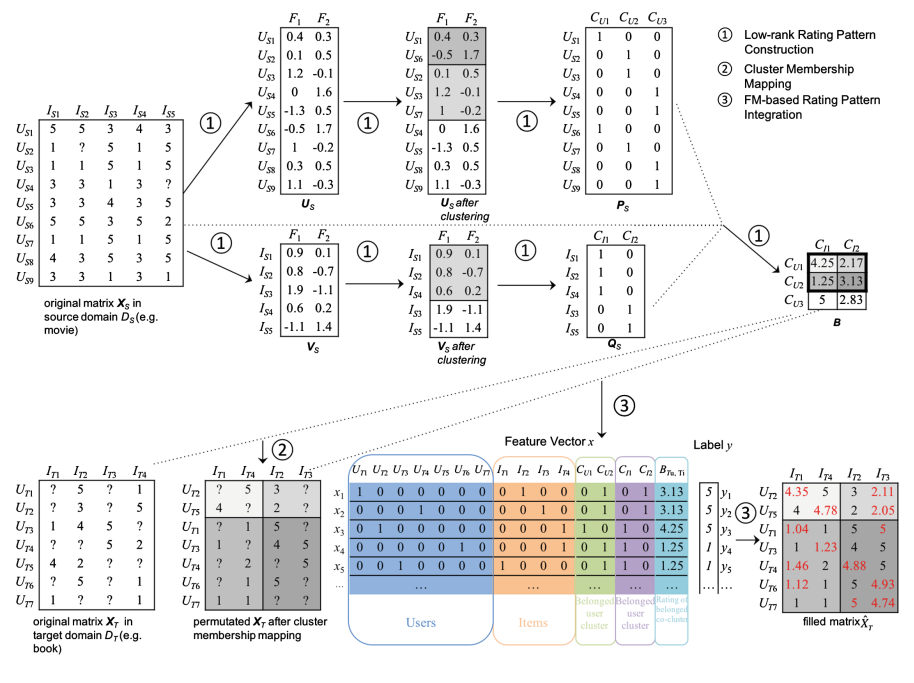
\includegraphics[width=\textwidth]{pictures/lkt-fm}
  \caption
  [Representation of the LKT-FM model. Source: https://doi.org/10.1007/978-3-319-71246-8\_39]
  {\protect\raggedright Representation of the LKT-FM model. Source: https://doi.org/10.1007/978-3-319-71246-8\_39}
\end{figure}